% results_human_comparison.tex
\subsection{Semantic--Behavioral Coherence}

Cleaning the human benchmark (see Method) left 874{,}434 of
1{,}015{,}341 respondents, the 18 reverse-keyed items rescored
($6 - x$) for keyed analyses:

{\scriptsize
\begin{verbatim}
> keep <- rowSums(human_raw < 1 | human_raw > 5 | is.na(human_raw)) == 0
> human <- human_raw[keep, ]
> cat("Respondents after cleaning:", n_human, "of", nrow(human_raw), "\n")
Respondents after cleaning: 874434 of 1015341
> human_fa <- psych::fa(R_human, nfactors = 5, n.obs = n_human,
+                       rotate = "oblimin", fm = "minres")
\end{verbatim}
}

Five factors were fixed a priori \citep{goldberg-1990}; parallel
analysis suggested up to ten---at $N = 874{,}434$ even trivial factors
clear noise---but five reproduced the Big Five with simple structure
(Table~\ref{tab:s-human-loadings}).

\subsubsection{Factor-Level Congruence}

\texttt{sfa\_congruence()} takes a fitted \texttt{psych} model as the
target:

{\scriptsize
\begin{verbatim}
> cong_human <- sfa_congruence(fit, target = human_fa,
+                              metrics = c("tucker", "nmi", "ari", "frobenius"))
> cong_human
Factor structure congruence

Tucker phi (factor-by-factor):
     MR4   MR1  MR3  MR2  MR5
MR3 0.03  0.80 0.30 0.13 0.12
MR1 0.27  0.11 0.10 0.84 0.28
MR2 0.41 -0.01 0.52 0.05 0.27
MR5 0.64  0.07 0.52 0.11 0.16
MR4 0.18  0.02 0.17 0.14 0.92

  NMI:            0.527 (moderate - higher is better)
  ARI:            0.402 (weak - higher is better)
  Frobenius:      0.664 (moderate - higher is better)
\end{verbatim}
}

Each semantic factor found a distinct human counterpart
(Table~\ref{tab:tucker}): Openness, Conscientiousness, and Neuroticism
strongly ($\phi = .92$, .84, .80); Extraversion (.64) and Agreeableness
(.52) weakly, the former matching human Agreeableness nearly as well
(.52). Overall, $\bar{\phi} = .744$, NMI = .527, ARI = .402, and
normalized Frobenius similarity .664 between the correlation
structures.

\begin{table}[H]
\centering
\captionsetup{justification=raggedright,singlelinecheck=false}
\caption{Tucker congruence coefficients between the semantic factors
(rows) and the human-response factors (columns)}
\label{tab:tucker}
\begin{tabular}{lrrrrr}
\toprule
& \multicolumn{5}{c}{Human factor} \\
\cmidrule(lr){2-6}
Semantic factor & E (MR4) & N (MR1) & A (MR3) & C (MR2) & O (MR5) \\
\midrule
N (MR3) & .03 & \textbf{.80} & .30 & .13 & .12 \\
C (MR1) & .27 & .11 & .10 & \textbf{.84} & .28 \\
A (MR2) & .41 & $-$.01 & \textbf{.52} & .05 & .27 \\
E (MR5) & \textbf{.64} & .07 & .52 & .11 & .16 \\
O (MR4) & .18 & .02 & .17 & .14 & \textbf{.92} \\
\bottomrule
\end{tabular}
\caption*{\textit{Note}. E = Extraversion; N = Neuroticism; A =
Agreeableness; C = Conscientiousness; O = Openness. MR labels are the
rotation-order factor names from each solution. Bold values mark each
semantic factor's best-matching human factor (mean matched
$\bar{\phi} = .744$). Semantic solution: minres/oblimin on the
mean-centered Pearson similarity matrix; human solution: minres/oblimin on
keyed response correlations, $N = 874{,}434$.}
\end{table}

\subsubsection{Comparing the Encodings}

Table~\ref{tab:encodings} extends this to every encoding's five-factor
solution; the NLI matrix, supplied via \texttt{similarity =}, was
indefinite (minimum eigenvalue $-14.1$), requiring positive-definite
projection (see Method).

\begin{table}[H]
\centering
\captionsetup{justification=raggedright,singlelinecheck=false}
\caption{Encoding comparison: congruence with theory, with the human factor
solution, and with human item-pair correlations, plus fit diagnostics}
\label{tab:encodings}
{\footnotesize
\setlength{\tabcolsep}{3.6pt}
\begin{tabular}{lrrrrrrrrrr}
\toprule
& \multicolumn{2}{c}{Theory} & \multicolumn{4}{c}{Human data} &
\multicolumn{4}{c}{Diagnostics} \\
\cmidrule(lr){2-3} \cmidrule(lr){4-7} \cmidrule(lr){8-11}
Encoding & NMI & ARI & $\bar{\phi}$ & $r_{\text{keyed}}$ &
$r_{\text{raw}}$ & $r_{\text{dis}}$ & KMO & TEFI & RMSR & CAF \\
\midrule
atomic                  & .527 & .402 & .744 & .434 & .456 & .707 & .971 & $-27.72$ & .032 & .412 \\
atomic\_reversed        & .527 & .402 & .438 & .137 & .444 & ---  & .971 & $-27.72$ & .032 & .412 \\
squid                   & .391 & .272 & .636 & .567 & .490 & 1.000 & .022 & $-44.39$ & .072 & .996 \\
mean\_centered\_pearson & .527 & .402 & .744 & .434 & .456 & .707 & .971 & $-27.71$ & .032 & .412 \\
nli                     & .548 & .448 & .310 & .063 & .561 & ---  & .551 & $-54.15$ & .094 & .688 \\
\bottomrule
\end{tabular}
}
\caption*{\textit{Note}. NMI = normalized mutual information and ARI =
adjusted Rand index of the five-factor item clustering against the
theoretical Big Five partition; $\bar{\phi}$ = mean Tucker congruence after
matching each semantic factor to its best human factor;
$r_{\text{keyed}}$ / $r_{\text{raw}}$ = correlation between the encoding's
1,225 item-pair similarities and the human inter-item correlations computed
from keyed and raw responses, respectively; $r_{\text{dis}}$ =
disattenuated congruence against the keyed human correlations. Dashes mark
cases where the disattenuated metric is undefined and reported as NA
because the similarity matrix's split-half reliability is not positive: the
keying flip of \texttt{atomic\_reversed} imposes a checkerboard sign
pattern (the signed NLI matrix behaves analogously). KMO, TEFI, RMSR, and
CAF are the fit diagnostics of each encoding's five-factor solution.}
\end{table}

Three patterns stand out. First, \texttt{atomic\_reversed}---an
anti-topic vector, not reverse-scoring's analogue (see
Discussion)---aligned worst among cosines with keyed correlations
($r_{\text{keyed}} = .137$ vs.\ .434 unflipped) and ordinarily only
with raw ($r_{\text{raw}} = .444$).

Second, NLI mirrors the cosines: best on the theoretical partition
(NMI = .548, ARI = .448) and on raw pairwise correlations
($r_{\text{raw}} = .561$), worst on loading shape
($\bar{\phi} = .310$), cosine the reverse ($\bar{\phi} = .744$,
$r_{\text{raw}} = .456$)---directional entailment versus graded
geometry (see Discussion).

Third, SQuID won keyed pair-level agreement ($r_{\text{keyed}} = .567$;
$r_{\text{dis}}$ saturated at 1.000) yet was essentially unfactorable
(KMO = .022), its differencing keeping pairwise relations but
stripping extractable common variance. Only keying-free
mean-centered Pearson combined near-best theory congruence (within
.021 NMI), the best loading-shape match ($\bar{\phi} = .744$), and a
genuine, well-conditioned correlation matrix (KMO = .971)---hence the
main fit.

\subsubsection{Item-Pair Agreement}

Across all 1,225 item pairs, structure from language alone matched the
raw correlations of 874{,}434 respondents at $r = .46$
(Figure~\ref{fig:semantic-human}).

\begin{figure}[H]
\centering
\captionsetup{justification=raggedright,singlelinecheck=false}
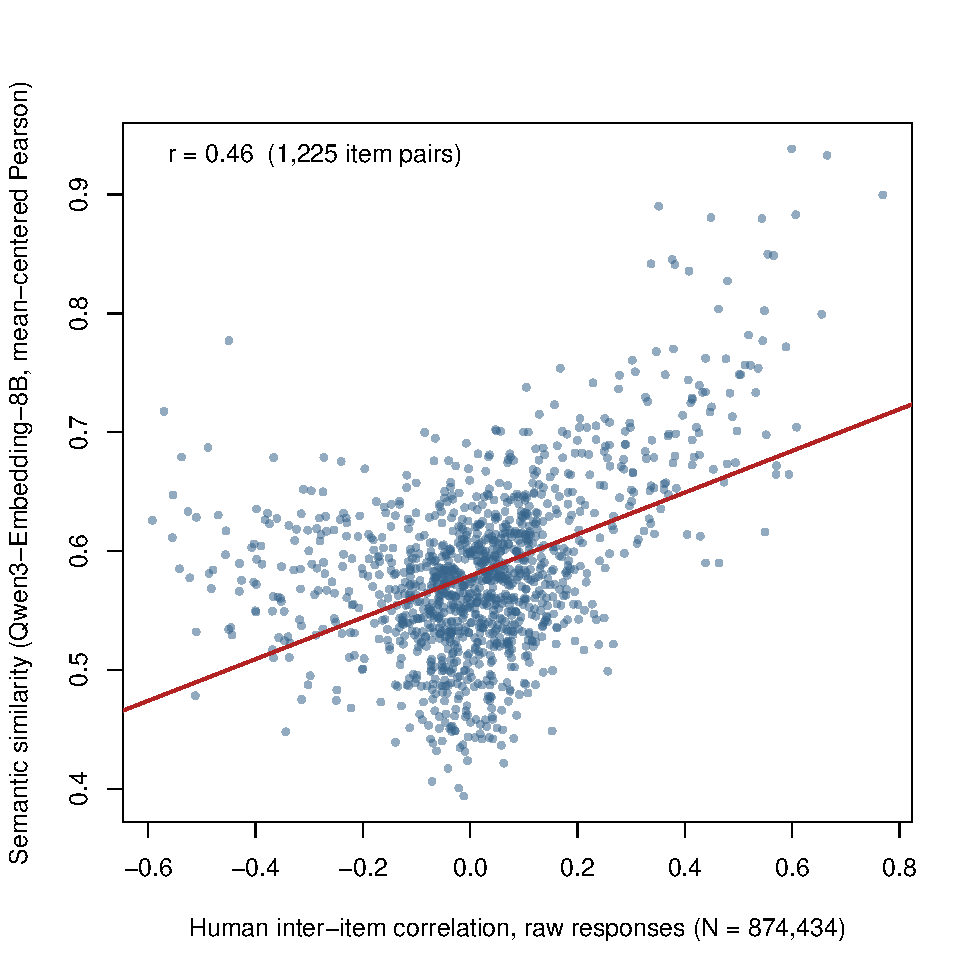
\includegraphics[width=0.6\textwidth]{figures/semantic_vs_human.pdf}
\caption{Semantic similarity (mean-centered Pearson encoding of the
Qwen3-Embedding-8B item vectors) against human inter-item correlations
from raw responses ($N = 874{,}434$), for all 1,225 item pairs;
$r = .46$. The fitted regression line is shown in red.}
\label{fig:semantic-human}
\end{figure}

Semantic--behavioral coherence is thus a measured relation: strong
convergence for three domains, partial where warmth--sociability
language blurs a boundary response covariance keeps sharp, and
informative, encoding-specific divergence where the similarity model
redefines ``meaning the same thing.''
